\que{Векторное произведение, его свойства, символы Леви-Чивиты.}
\begin{definition}[Символ Леви-Чивиты]
	\begin{equation*}
		\epsilon_{ijk},\epsilon^{ijk} = \begin{cases}
			0, &\text{если среди $i,j,k$ есть повторения};\\
			1, &\text{если $(ijk)$ - четная подстановка};\\
			-1,&\text{если $(ijk)$ - нечетная подстановка}.\\
		\end{cases}
	\end{equation*}
\end{definition}

\begin{definition}[Определитель]
	Для матрицы 3х3 верна формула:
	\begin{equation*}
		\det(\tensor{A}{^i_j}) = \frac{1}{6}\epsilon_{ijk}\epsilon^{mnl}\tensor{A}{^i_m}\tensor{A}{^j_n}\tensor{A}{^k_l}.
	\end{equation*}
	(легко можно проверить подставив в лоб)
	
	Расписав покомпонентно один из символов Леви-Чевиты и упростив легко выделить другое выражение
	\begin{equation*}
		\det(\tensor{A}{^i_j}) = \epsilon_{ijk}\tensor{A}{^i_\alpha}\tensor{A}{^j_\beta}\tensor{A}{^k_\gamma},\quad \alpha\neq\beta\neq\gamma,\quad\alpha,\beta,\gamma=1,2,3.
	\end{equation*}
\end{definition}

Для метрической матрицы $g_{ij}, g^{ij}$ формулы выше также применимы, тогда получим, что:
\begin{align*}
	g &= \frac{1}{6}\epsilon^{ijk}\epsilon^{mnl}g_{mi}g_{nj}g_{kl},\\
	\sqrt{g}\epsilon_{ijk}&=\frac{1}{\sqrt{g}}\epsilon^{mnl}g_{mi}g_{nj}g_{lk}.
\end{align*}

\begin{definition}[Векторное произведение]
	Векторным произведением векторов $\mathbf{a}, \mathbf{b}$ из $\mathcal{E}_3$ называют следующий вектор $\mathbf{c}$ из $\mathcal{E}_3$:
	\begin{equation*}
		\mathbf{c} = \mathbf{a} \times \mathbf{b} = \sqrt{g} \epsilon_{ijk} a^ib^j\mathbf{e}^k = \frac{1}{\sqrt{g}}\epsilon^{ijk} a_ib_j\mathbf{e}_k
	\end{equation*}
\end{definition}

\begin{theorem}
	Для векторного произведения имеет место формула 
	\begin{equation*}
		\mathbf{a} \times \mathbf{b} = S\mathbf{n},
	\end{equation*}
	\begin{equation*}
		S = |\mathbf{a}||\mathbf{b}|\sin{\varphi},
	\end{equation*}
	где $\varphi$ угол между $\mathbf{a}$ и $\mathbf{b}$ ($0\leqslant\varphi\leqslant\pi$), а $\mathbf{n}$ единичный вектор, ортогональный к $\mathbf{a}$ и $\mathbf{b}$. Иллюстрация, см. Рисунок \ref{fig:que5}.
	
	\begin{proof}
		Если один из векторов $\mathbf{a}$ и $\mathbf{b}$ нулевой, то формула, очевидно, выполняется. Если векторы $\mathbf{a}$ и $\mathbf{b}$ коллинеарны, то же самое. Рассмотрим случай, когда $\mathbf{a}$ и $\mathbf{b}$ ненулевые и неколлинеарные.
		
		$\mathbf{a}$ и $\mathbf{b}$ ненулевые и неколлинеарные. Построим базис $\mathbf{e}'_i$ в $E_2$:
		\begin{equation*}
			\mathbf{e}'_1 = \mathbf{a},\quad\mathbf{e}'_2=\mathbf{b},\quad\mathbf{e}'_3=\mathbf{n}
		\end{equation*}
		Компоненты векторов $\mathbf{a}$ и $\mathbf{b}$ в этом базисе:
		\begin{equation*}
			a'i=\begin{pmatrix}
				1\\0\\0
			\end{pmatrix},\quad
			b'i=\begin{pmatrix}
				0\\1\\0
			\end{pmatrix},
		\end{equation*}
		а метрическая матрица:
		\begin{equation*}
			g'_{ij}=\mathbf{e}'_i\cdot\mathbf{e}'_j=\begin{pmatrix}
				|\mathbf{a}|^2            & \mathbf{a}\cdot\mathbf{b} & 0 \\
				\mathbf{a}\cdot\mathbf{b} & |\mathbf{b}|^2            & 0 \\
				0                         & 0                         & 1
			\end{pmatrix}
		\end{equation*}
		Тогда
		\begin{equation*}
			S=\sqrt{g'_{11}g'_{22}}\sin{\varphi}=\sqrt{g'_{11}g'_{22}}\sqrt{1-\cos^2{\varphi}},
		\end{equation*}
		где
		\begin{equation*}
			\cos\varphi = \frac{\mathbf{a}\cdot\mathbf{b}}{|\mathbf{a}||\mathbf{b}|}=\frac{g'_{12}}{\sqrt{g'_{11}g'_{22}}}, \quad\sqrt{1-\cos^2{\varphi}} = \sqrt{\frac{g'}{g'_{11}g'_{22}}}.
		\end{equation*}
		Таким образом
		\begin{equation*}
			S = \sqrt{g'_{11}g'_{22}}\sqrt{\frac{g'}{g'_{11}g'_{22}}} = \sqrt{g'},
		\end{equation*}
		При этом имеем
		\begin{equation}\label{vec prod}
			\mathbf{a} \times \mathbf{b} = \sqrt{g'} \epsilon_{123} a'^1b'^2\mathbf{e}'^3=\sqrt{g'}e'^3
		\end{equation}
		Подставляя в \eqref{vec prod} всё имеющееся, действительно получаем
		\begin{equation*}
			\mathbf{a} \times \mathbf{b} = S\mathbf{n}.
		\end{equation*}
	\end{proof}
\end{theorem}
\begin{figure}[ht!]
	\centering
	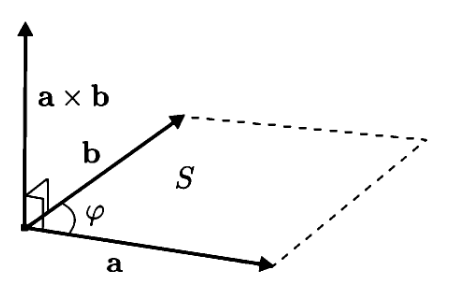
\includegraphics[width=0.5\linewidth]{img/que5}
	\caption{Геометрическое изображение векторного произведения в пространстве $E_3$}
	\label{fig:que5}
\end{figure}
\begin{theorem}[О связи векторов взимного и основного базисов в $\mathcal{E}_3$]
	Векторы взимного и основного базисов в $\mathcal{E}_3$ связаны с помощью операции векторного произведения:
	\begin{equation*}
		\mathbf{e}^\gamma = \frac{1}{\sqrt{g}}\mathbf{e}_\alpha\times\mathbf{e}_\beta,\quad\mathbf{e}_\gamma=\sqrt{g}\mathbf{e}^\alpha\times\mathbf{e}^\beta,\quad \alpha\neq\beta\neq\gamma,\quad\alpha,\beta,\gamma=1,2,3.
	\end{equation*}
	\begin{proof}
		\begin{equation*}
			\mathbf{e}_n\times\mathbf{e}_m=\sqrt{g}\epsilon_{ijk}\delta^i_n\delta^j_m\mathbf{e}^k=\sqrt{g}\epsilon_{nmk}\mathbf{e}^k
		\end{equation*}
	\end{proof}
\end{theorem}
